\chapter{Communication}

\begin{flushleft}
  \begin{minipage}[t]{0.47\linewidth}
    \raggedright
    The communication between components can be implemented in different ways:

    \begin{itemize}
      \item Local vs Distributed
      \item Synchronous vs Asynchronous
      \item One-to-one vs One-to-many
      \item One-way vs Two-way
      \item Call vs Message vs Shared memory
    \end{itemize}
  \end{minipage}%
  \hfill
  \begin{minipage}[t]{0.47\linewidth}
    \raggedright
    There are some distributed computing fallacies that are worth mentioning:

    \begin{enumerate}

      \item The network is reliable;
      \item Latency is zero;
      \item Bandwidth is infinite;
      \item The network is secure;
      \item Topology doesn't change;
      \item There is one administrator;
      \item Transport cost is zero;
      \item The network is homogeneous.

    \end{enumerate}
  \end{minipage}
\end{flushleft}

\paragraph{Network latency} - Due to decomposition an operation may result into
a series of round-trips between two services.
Some solution can be: Batch API that allow feeding multiple
requests or merge services to convert messages to
method calls,


\begin{table}[h!]
  \renewcommand{\arraystretch}{1.4}
  \centering
  \begin{tabular}{l c c}
    \toprule
                           & \multicolumn{2}{c}{\textbf{Multiplicity}}                        \\
                           & \textbf{One-to-one}                       & \textbf{One-to-many} \\
    \midrule
    \textbf{Sync}          & Request/response                          & --                   \\
    \textbf{Async One-way} & Notification                              & Publish/Subscribe    \\
    \textbf{Async Two-way} & Async. Req./Resp.                         & Publish/Async. Resp. \\
    \bottomrule
  \end{tabular}
\end{table}


\subsection{One-to-one communication}

\begin{itemize}

  \item \textbf{Request-response} - A client makes a request to a service and waits
        for a response. The client blocks while waiting.

  \item \textbf{Asynchronous request/response} - A client sends a request to a
        service, which replies asynchronously. The client doesn't block while waiting.

  \item \textbf{One-way notifications} - A client sends a request to a service, but no
        reply is expected or sent.

\end{itemize}

\subsection{One-to-many communication}

\begin{itemize}

  \item \textbf{Publish/subscribe} - A client publishes a notification message, which
        is consumed by zero or more interested services.

  \item \textbf{Publish/async. response} - A client publishes a request message and
        then waits for a certain amount of time for responses from interested services.

\end{itemize}

\section{Messaging}
Messages are exchanged over message channels. A sender writes a message to a
channel, and a receiver reads messages from a channel. The communication is
asynchronous, the sender doesn't block waiting for a reply

\paragraph{Header}
The header contains metadata about the message, such as: Message ID, Return address, Metadata that describes the content of the message, Collection of key-value pairs useful for routing, filtering, etc.

\paragraph{Body}
The body contains the data being sent in either text or binary format.

\subsection{Message types}

\begin{itemize}

  \item \textbf{Command} - This is equivalent of an RPC request. It specifies the
        operation to invoke and its parameters.

  \item \textbf{Document} - Contains only data. The receiver decides how to interpret
        it, e.g. a reply to a command

  \item \textbf{Event} -  Indicates that something notable has occurred. An event is
        often a domain event, which represents a state change of a domain object.

\end{itemize}

\section{Channel}

\subsection{Point-to-point channels}
Delivers a message to exactly one of the
consumers that is reading from the channel.

Services use point-to-point channels for the one-
to-one interaction styles. E.g. command messages

\subsection{Publish-subscribe channels}

Channel delivers each message to all of the attached consumers.
Services use publish-subscribe channels for the
one-to-many interaction styles


\begin{center}
  \begin{minipage}{0.8\linewidth}
    \begin{minipage}{0.48\linewidth}
      \centering
      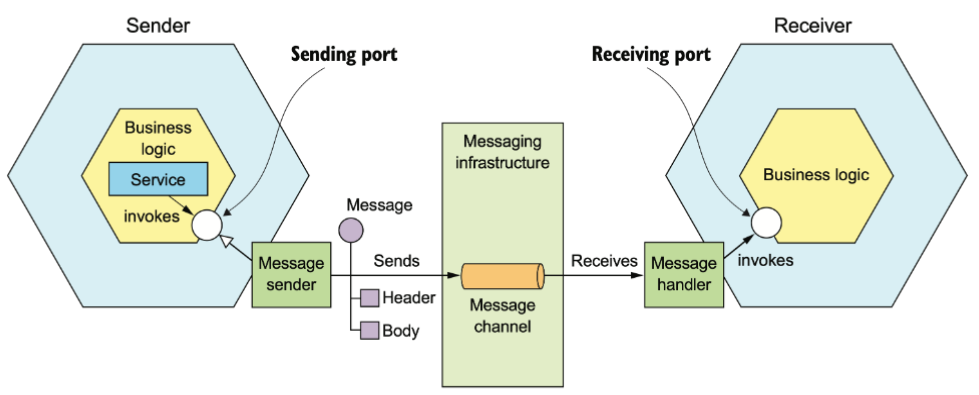
\includegraphics[width=0.8\linewidth]{content/chapters/images/2026-04-11-10-58-16.png}
    \end{minipage}%
    \hfill
    \begin{minipage}{0.48\linewidth}
      \centering
      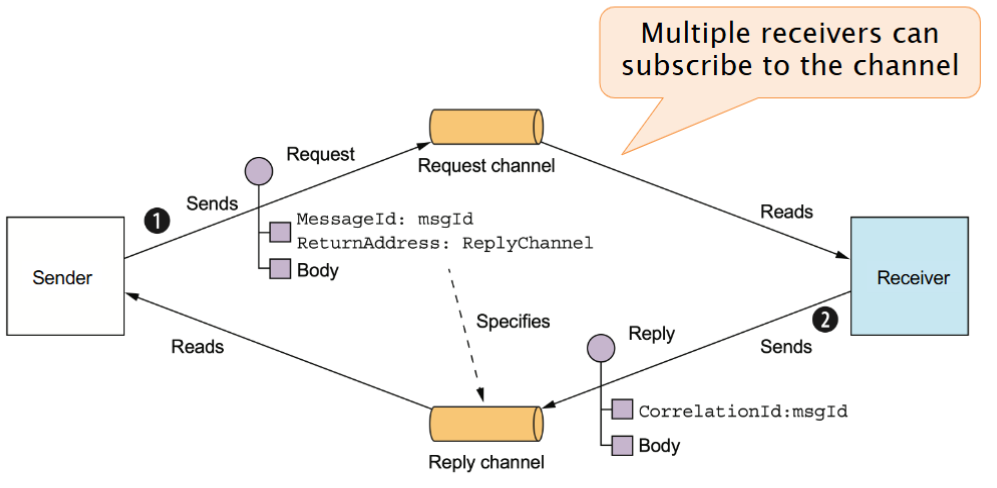
\includegraphics[width=0.8\linewidth]{content/chapters/images/2026-04-11-10-59-30.png}
    \end{minipage}
  \end{minipage}
\end{center}


\section{Supported styles}

\begin{itemize}
  \item Request/response - supports synchronous or asynchronous
  \item One-way notification - No response
  \item Publish/subscribe - Multiple subscribers no response
  \item Publish/Async responses - Multiple subscribers, multiple responses
\end{itemize}

\section{Direct messaging - brokerless}


\begin{table}[h!]
  \renewcommand{\arraystretch}{1.4}
  \centering
  \begin{tabular}{ll}
    \toprule
    \textbf{Pros}                      & \textbf{Cons}                                                 \\
    \midrule
    Lighter traffic load, less latency & Services must be known $to$ discovery                         \\
    No centralized point of failure    & Reduced availability, both must be available at the same time \\
    Simplicity                         & Hard to have guaranteed delivery                              \\
    \bottomrule
  \end{tabular}
\end{table}


\section{Broker-based messaging}

Broker is an intermediary components through which all messages flow.

\begin{table}[h!]
  \renewcommand{\arraystretch}{1.4}
  \centering
  \begin{tabular}{ll}
    \toprule
    \textbf{Pros}                                               & \textbf{Cons}                    \\
    \midrule
    Loose coupling.                                             & Potential performance bottleneck \\
    No need to know each other or to be active at the same time & Single point of failure          \\
                                                                & Additional complexity            \\
    \bottomrule
  \end{tabular}
\end{table}



\subsection{Broker characteristics}

It support both standard protocols, e.g. AMQP, MQTT, STOMP, or proprietary protocols.
It has some good feature such as:

\begin{itemize}
  \item Messaging ordering
  \item Guaranteed delivery
  \item Persistence
  \item Durability, consumer can disconnect and reconnect without losing messages
  \item Scalability
  \item End-to-end latency
  \item Support for cometing consumers
\end{itemize}


\section{Coordination}

\subsection{Choreography}

Each local transaction publishes domain
events that trigger local transactions in
other services.

\begin{flushleft}
  \begin{minipage}{0.55\linewidth}
    \raggedright
    \begin{itemize}
      \item It requires reliable message infrastructure and messages with correlation id.
      \item Basic operation is simple, it perform operation and publish event
      \item Difficult to understand and maintain because transaction logic is scattered
      \item Complex service dependencies also cyclic, might lead to tight coupling
    \end{itemize}
  \end{minipage}%
  \hfill
  \begin{minipage}{0.37\linewidth}
    \centering
    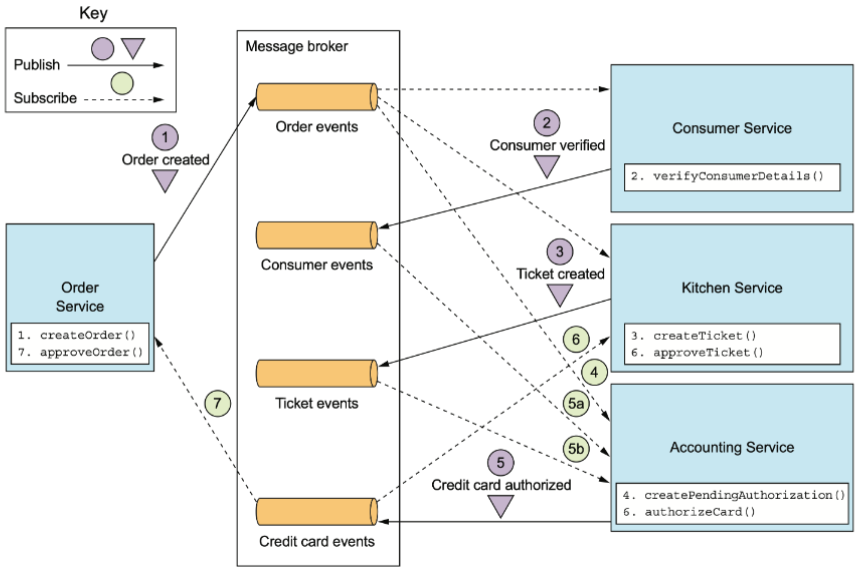
\includegraphics[width=\linewidth]{content/chapters/images/2026-04-11-11-16-28.png}
  \end{minipage}
\end{flushleft}

\subsection{Orchestration}
An orchestrator (object) tells the
participants what local transactions to
execute.

This teqnique requires reliable messaging, it has a simple dependency structure with
reduced coupling.

The business logic is simple and services are not aware of the saga.
Transaction logic is gathered in a single place, must be kept separate from service logic.


\begin{center}
  \begin{minipage}{0.45\linewidth}
    \centering
    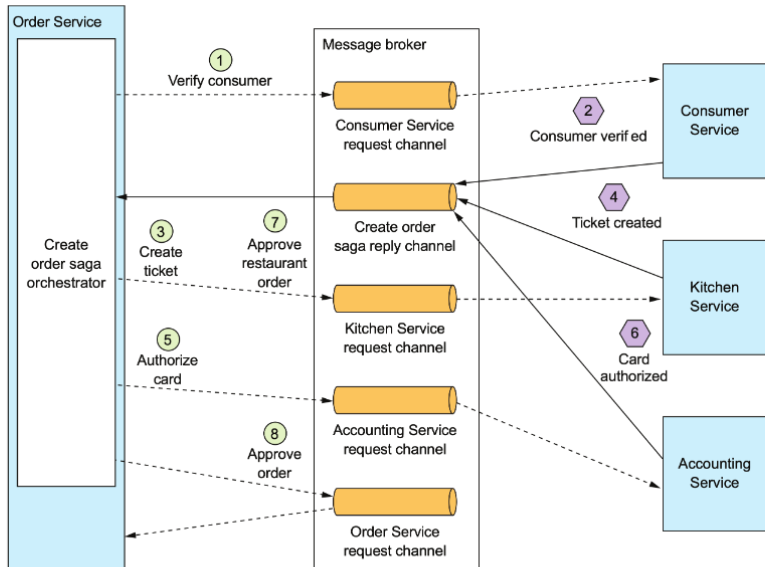
\includegraphics[width=0.7\linewidth]{content/chapters/images/2026-04-11-11-20-19.png}
  \end{minipage}%
  \hfill
  \begin{minipage}{0.45\linewidth}
    \centering
    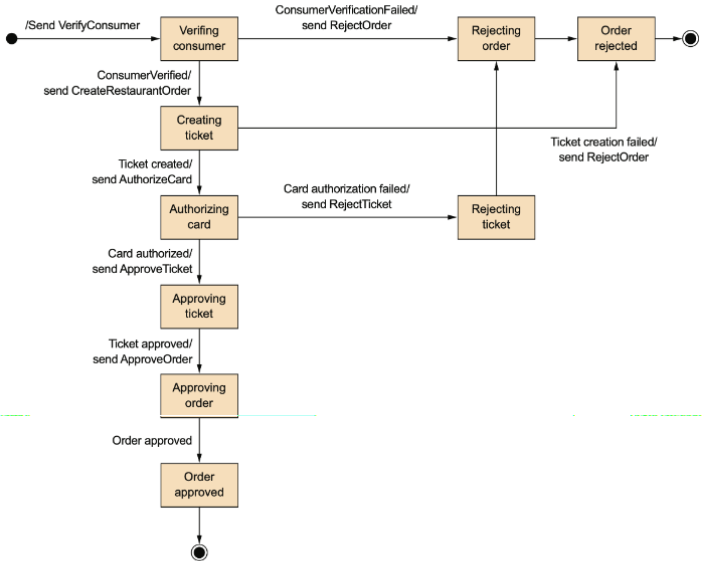
\includegraphics[width=0.7\linewidth]{content/chapters/images/2026-04-11-11-20-44.png}
  \end{minipage}
\end{center}





